\documentclass[12pt, a4paper]{article}

\usepackage{fontspec}
\usepackage{xcolor}
\usepackage{pgfgantt}
\usepackage{tikz}
\usepackage{authblk}
\usepackage{bookmark}
\usepackage{booktabs}
\usepackage[section]{placeins}
\usepackage{hyperref}

\hypersetup{
    colorlinks=false,
    pdfborder={0 0 0},
}
\setmainfont{Noto Sans Condensed}

\setlength{\parindent}{0pt}
\setlength{\parskip}{0.5\baselineskip}

%\definecolor{nordblue}{RGB}{129, 161, 193}
\definecolor{nordblue}{RGB}{94, 129, 172}
\definecolor{nordyellow}{RGB}{235,203,139}

%\backgroundsetup{%
%  scale=1,
%  color=black,
%  opacity=0.2,
%  angle=0,
%  contents={%
%    \includegraphics[width=\paperwidth,height=\paperheight]{magnolia.png}
%  }
%}

\title{\Huge{Gypsophino}}
\author{Group 27}
\date{}

\begin{document}
\begin{titlepage}
  \maketitle
\end{titlepage}

\tableofcontents
\clearpage

\section{Group Number}

Group 27

\section{Group Members}

\begin{table}[h]
  \centering
  \begin{tabular}{cc}
    \toprule
    Student Name & Student ID\\
    \midrule
    Haoxiang Fei & 519370910099\\
    Qin Huang & 519021910485\\
    Simin Wang & 519370910102\\
    \bottomrule
  \end{tabular}
\end{table}

\section{Project Name}

Gypsophino

\section{Intended Language}

C++

\section{Summary}

Our project is a kind of music game that can be played on the computer.

\section{Motivation}

We want to design our own music game because all members in our group love music.
And we'd like to have some new with music games in general, such as pixel blocks with a major tone and a new storyline.

\section{Tentative Design}

\subsection{Features}

\subsubsection{Note Hitting}

Our software is designed to provide player a basic, intuitive
music game playing experience. And the core function of a music game
is note hitting. Colorful notes will fall down from above, and player
need to press down certian keys on the keyboard at certain instant of time
to get points.

\subsubsection{Music Map Management System}

Our software is designed to be capable to handle multiple music maps.
Player is allow to select the music map and play. Players can also
compose their own maps and share it with friends.

\subsubsection{Score System}

Our score system is designed to be able to calculate score for any single
valid hit of note and give the player instant feedback. The score system
is also able to store the history score of the player.

\subsubsection{Settings}

Default settings of the falling speed of the notes and the offset may not
fits everyone well, so player can modify these basic settings and volume
of the effect sound and the music in our software.

\subsubsection{Different Difficulties}

One difficulties of a piece of music is not enough. Our software should
be friendly to the new music gamer, and be challenging to experts.
A auto difficulties multiplexer may be also include to reduce the workload
of map writers.

\subsubsection{Story Line}

Pure music game might be too hardcore. A music game with story might be
oriented to a larger group of people. Our story system can have
multiple branch according to players choices and performance in playing.
And it is also has multiple ends waiting for players to explore.

\subsubsection{Mod System}

Our game allows player to develop and use mod to create additional
content of the story, or re-organize the note arrangement of maps
to more challenging or more easy, etc.

\subsubsection{Multiple Player System}

Our game allows player to play this game with their friends locally.
Two players can also cooperate to finish a song.

\subsection{Diagram of Our Software}

\begin{figure}[h]
  \centering
  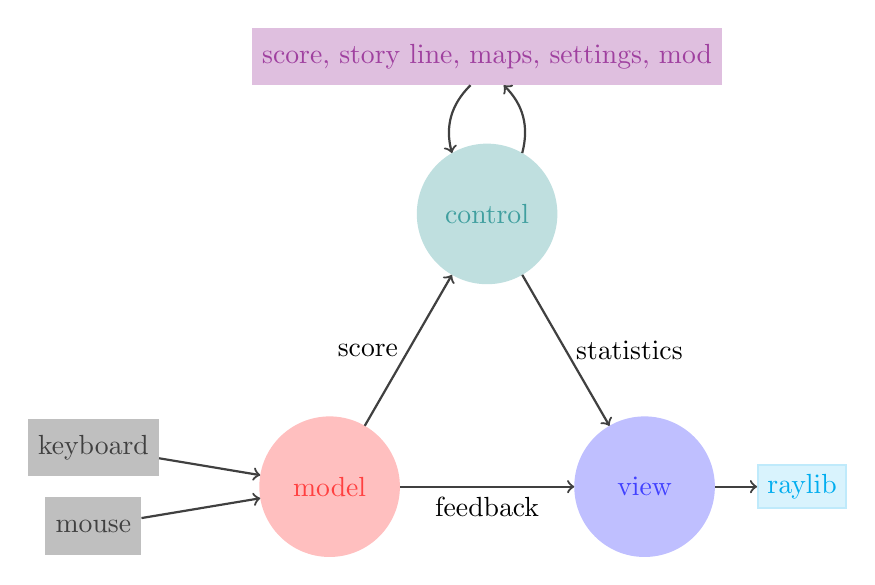
\begin{tikzpicture}
    \node (model) [circle, thick, draw=red!25, fill=red!25, text=red!75, minimum size=50] at (-2, -1.732) {model};
    \node (control) [circle, thick, draw=teal!25, fill=teal!25, text=teal!75, minimum size=50] at (0, 1.732) {control};
    \node (view) [circle, thick, draw=blue!25, fill=blue!25, text=blue!75, minimum size=50] at (2, -1.732) {view};
    \node (keyboard) [rectangle, thick, draw=black!25, fill=black!25, text=black!75, minimum size=20] at (-5, -1.232) {keyboard};
    \node (mouse) [rectangle, thick, draw=black!25, fill=black!25, text=black!75, minimum size=20] at (-5, -2.232) {mouse};
    \node (cglib) [rectangle, thick, draw=cyan!25, fill=cyan!15, text=cyan] at (4, -1.732) {raylib};
    \node (db) [rectangle, thick, draw=violet!25, fill=violet!25, text=violet!75, minimum size=20] at (0, 3.732) {score, story line, maps, settings, mod};
    \draw [->, thick, draw=black!75] (keyboard) edge (model);
    \draw [->, thick, draw=black!75] (mouse) edge (model);
    \draw [->, thick, draw=black!75] (view) edge (cglib);
    \draw [->, thick, draw=black!75, bend right] (control) edge (db);
    \draw [->, thick, draw=black!75, bend right] (db) edge (control);
    \draw [->, thick, draw=black!75] (model) edge node[left] {score} (control);
    \draw [->, thick, draw=black!75] (model) edge node[below] {feedback} (view);
    \draw [->, thick, draw=black!75] (control) edge node[right] {statistics} (view);
  \end{tikzpicture}
\end{figure}

\section{Expected Outcome}

\subsection{Bottom-line}

\begin{enumerate}
  \item basic operating of a rhythm game
  \item score system
  \item basic settings (volume)
  \item ability to import pre-composed map (manually)
  \item cover picture
\end{enumerate}

\subsection{Expected}

\begin{enumerate}
  \item story line
  \item plot pictures (CGs)
  \item difficulty level
  \item advanced settings (user can customize the offset between the music and graphics according to their experience)
\end{enumerate}

\subsection{Potential}

\begin{enumerate}
  \item MODs (like invincible mode)
  \item Versus mode
\end{enumerate}


\section{Timetable}

\begin{ganttchart}[
  canvas/.style={draw=none},
  title/.style={fill=teal!20, draw=teal!20},
  title label font=\color{teal}\bfseries,
  today=0,
  today rule/.style={draw=teal, thick, dashed},
  expand chart=\textwidth,
  bar label node/.append style={align=left,text width=12em},
  bar/.append style={fill=nordblue, draw=none},
  bar incomplete/.append style={fill=teal!20},
  progress label text={}
  ]{1}{5}
  \gantttitle{Week}{5}\\
  \gantttitlelist[
  title/.style={draw=teal!20, fill=teal!20}
  ]{1,2,3,4,5}{1}\\
  \ganttbar[progress=0]{Note Hitting}{1}{2}\\
  \ganttbar[progress=0]{Score \& Settings}{2}{3}\\
  \ganttbar[progress=0]{Map System \& Difficulties}{3}{4}\\
  \ganttbar[progress=0]{Story Line \& Art}{1}{5}\\
  \ganttbar[progress=0]{Mod System \& PvP}{3}{5}\\
\end{ganttchart}

\section{Extra Perparations}

To process the incoming keystorks while drawing,
we need to learn the knowledge about the asynchronous communication and
multi-threads.

To write well-structured code, we need to learn some software engineering
method like OOP\@.

To draw graphics, we need to learn that how to use OpenGL or other
computer graphics library/framework.

Since our members don't share the same operating system, we need to have
a basic understanding of the platform compatibility.

As we need to manager the maps and track the game score, we need to learn
the organization and the basic usage of the database.

\section{Task Assignment}

\paragraph{Fei HaoXiang}
\begin{enumerate}
  \item Note hitting
  \item Advanced settings
  \item Versus mode
\end{enumerate}

\paragraph{Wang Simin}
\begin{enumerate}
  \item Write story
  \item Basic settings and maps
  \item Maps system
  \item MODs
\end{enumerate}

\paragraph{Huang Qin}
\begin{enumerate}
  \item Draw cover and plot pictures
  \item Score system
  \item Set the beats 
  \item UI (including integration of stories and images)
\end{enumerate}

\end{document}

%Base:
%
%1. settings
%1. basic running of game
%1. 1-2 map
%1. score
%
%Expected:
%1. story line
%1. difficulties
%
%Potential:
%1. mod system
%1. 2p
